\chapter{Results}
\label{ch:results}

\Gls{fps} provided the core datasets required to conduct a preliminary routing analysis: school locations, schools served, school start times, student home locations, assigned schools, grade levels, current bus assignment, and fleet characteristics, including bus size, capacity, and type. \gls{fps} also confirmed that all buses operate from a single central depot and that current school transportation is planned independently of the local public transportation provider, \gls{mwrta}. Accordingly, \gls{mwrta} service is excluded from this analysis.

The available data is sufficient to identify and assess the current routing and test alternative configurations, but it is not yet sufficient for final implementation. The key limitation is that the dataset for currently served students includes assigned stops and disability status, but these records cannot be directly linked to each student's home address. This prevents full validation of current stop assignments and limits the precision of student-level service comparisons. I estimate Census-based demographic information by determining the corresponding block-group for different student addresses, then randomly sampling based on the percentage returned from \gls{acs} 5-year estimates.

\begin{table}[!htbp]
    \centering
    \begin{tabular}{@{}lll@{}}
    \toprule
        Category & Quantity & Avg Dist. to School [mi] \\ \midrule
        All students in \gls{fps} & 8210 & 2.81 \\
        Students currently riding bus & 4780 & 3.55 \\
        Within 1 mile of school & 1085 & 0.62 \\
        Within 2 miles of school & 2412 & 1.35 \\
        Further than 5 miles from school & 531 & 5.36 \\
        Language other than English at home & 4034 & 2.97 \\
        Non-car owning household & 760 & 3.03 \\
        Students with disabilities & 1096 & 2.49 \\ 
        \bottomrule
    \end{tabular}
    \caption{\gls{fps} student demographics and average home-to-school distance by student group, reported in miles. Categories are not mutually exclusive; a student may belong to multiple rows.}
    \label{tab:demographics}
\end{table}

\section{Existing Routes}
\label{sec:existing_routes}

Current routing is shaped by the interaction between district school choice policies and Massachusetts transportation requirements. Under Massachusetts General Laws (MGL Ch. 71, Section 68), districts must provide free transportation to K-6 students living more than 2 miles from school. As shown in \autoref{fig:geospatial}, this policy creates a clear incentive for some families in Framingham to select schools farther from home in order to secure transportation coverage. This pattern is especially visible among lower-income and minority households in the southern part of the city, as well as among families of students with disabilities.

\begin{figure}[!htbp]
    \centering
    \begin{subfigure}{0.33\textwidth}
        \subcaption{Students by distance to school}
        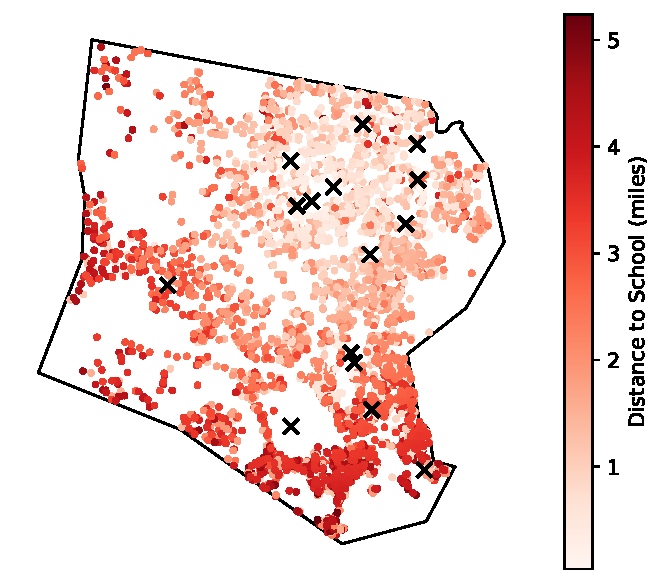
\includegraphics[width=0.99\textwidth, alt={Map of student locations in Framingham colored by distance to school. Darker red points indicate students farther from school, with schools marked by black X symbols.}]{figures/students_distance_to_school.pdf}
    \end{subfigure}
    \begin{subfigure}{0.33\textwidth}
        \subcaption{Location of students with disabilities}
        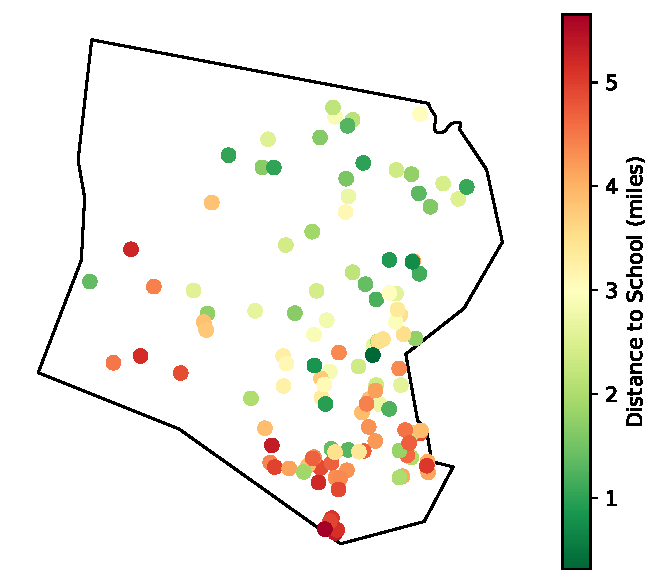
\includegraphics[width=0.99\textwidth, alt={Map of students with disabilities in Framingham colored by distance to school. Points show student locations, and warmer colors indicate longer school distances.}]{figures/special_education_students.pdf}
    \end{subfigure}
    \begin{subfigure}{0.33\textwidth}
        \subcaption{Median income by block group}
        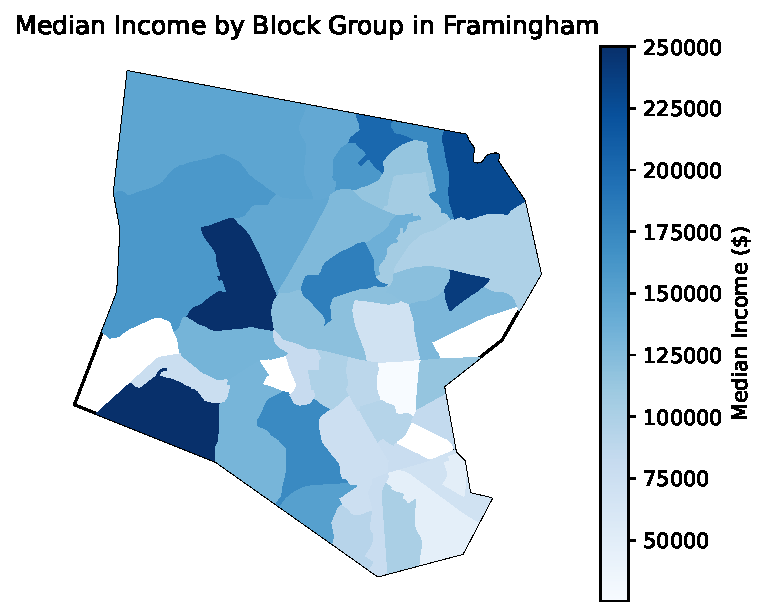
\includegraphics[width=0.99\textwidth, alt={Choropleth map of median income by census block group in Framingham. Darker blue areas indicate higher median income, and lighter areas indicate lower median income.}]{figures/median_income_by_block_group.pdf}
    \end{subfigure}
    \caption{Plots of different socioeconomic factors in Framingham, MA. Block groups from U.S. Census 2020.}
    \label{fig:geospatial}
\end{figure}

The current assignment therefore reflects both operational routing decisions and upstream policy-driven demand. At present, \gls{fps} uses 51 buses (with a maximum of 86 available) to serve 219 students with disabilities and 4,561 students without disabilities at the identified schools (4,780 riders total, matching \autoref{tab:demographics}).

\section{Experimental Methodology}

I use \gls{osm} to model the road network and connect it with existing depot, stop, and school locations. Based on walking distances computed using \textcite{fink2022R5py}, students are assigned to their closest stops (or for currently served students, impose the current assignment). Given the available bus fleet, school bell/start times, a manually set time window before these bell times, and a maximum in-vehicle ride-time (here set to 60 minutes), I then compute new routes based on the described \gls{bra}, adapting the decomposition approach of \textcite{bertsimasOptimizingSchoolsStart2019}. 

Because \gls{fps} was not yet able to provide real-world \gls{avl} data, \gls{bra} assumes a fixed driving speed of 30 miles per hour, incorporating boarding and alighting times of the various student groups (including students with disabilities, students requiring wheelchair-accessible routes, and students without additional transportation needs), and allows for multiple rounds by the same bus, dropping off students at one school before picking up additional students and bringing them to another school. To do so, this approach first allocates routes to students requiring accessible routes and students with disabilities, then caters to the remaining students.

\section{Currently Assigned Students}

The preliminary results indicate that \gls{bra} can improve \gls{fps}'s bus operations while preserving student coverage. Under the tested configuration, the algorithm serves the same 4,780 currently assigned students using 48 buses instead of 51, reducing deployed buses by 3, or approximately 5.9\%. This suggests that the existing network contains meaningful routing inefficiency that can be addressed through algorithmic reassignment and multi-school bus utilization. The core operational advantage of \gls{bra} is that it allows each bus to complete multiple trips across schools, while each trip remains structured around a specific grade and school assignment. For this preliminary test, I use conservative estimates and assume buses travel at an average speed of 30 miles per hour, require 30 seconds for student boarding, 1 minute for boarding students with disabilities, arrive between 10 minutes and 40 minutes before school bell time, and include a required 10-minute dwell time at the school as a buffer.

\begin{table}[!htbp]
    \centering
    \begin{tabular}{@{}lllllllll@{}}
        \toprule
        Category 
        & \multicolumn{4}{l}{\textbf{Current Routing}} 
        & \multicolumn{4}{l}{\textbf{BRA with Current Students}} \\
        & Mean & StDev & Min & Max 
        & Mean & StDev & Min & Max \\ 
        \midrule
        Currently assigned 
        & 43.08 & 29.00 & 3.05 & 133.38 
        & 30.52 & 14.13 & 1.64 & 58.31 \\
        Non-English at home 
        & 41.24 & 28.16 & 3.91 & 133.38 
        & 31.18 & 13.72 & 1.64 & 58.31 \\
        Non-car owning household 
        & 39.83 & 27.89 & 3.91 & 133.37 
        & 30.66 & 13.28 & 1.64 & 58.23 \\
        Students with disabilities
        & 36.68 & 20.82 & 3.05 & 125.38 
        & 25.35 & 13.33 & 2.14 & 57.86 \\
        \midrule
        Buses used 
        & \multicolumn{4}{l}{51} 
        & \multicolumn{4}{l}{48} \\
        \bottomrule
    \end{tabular}
    \caption{Estimated travel times in minutes for currently assigned riders under current routing versus the \gls{bra} configuration. Does not account for intersection delay, assumes constant bus speed.}
    \label{tab:travel_times}
\end{table}

The benefits are not limited to fleet utilization. Across all tracked student groups, \gls{bra} reduces estimated mean travel times relative to the current routing baseline, as shown in \autoref{tab:travel_times}. For currently assigned bus riders, mean travel time falls from 43.08 minutes to 30.52 minutes, a reduction of approximately 29.2\%, while the maximum observed travel time falls from 133.38 minutes to 58.31 minutes. 

Vulnerable groups also see consistent improvements under the modeling assumptions (\autoref{tab:travel_times}): mean travel time declines from 41.24 to 31.18 minutes for students from households where English is not the primary language, from 39.83 to 30.66 minutes for students from non-car-owning households, and from 36.68 to 25.35 minutes for students with disabilities. Additionally, because mean travel time decreased for non-car-owning households by approximately 23.0\% under \gls{bra}, this suggests that efficiency improvements are not achieved by sacrificing service to transit-dependent households. \autoref{fig:routes} shows the current and proposed route layouts side-by-side.

These findings are directional rather than final, since the analysis does not yet account for intersection delay, time-varying congestion, or all student-specific service requirements (e.g. wheelchair students due to missing data). Nonetheless, they establish a clear proof of concept: better route design can potentially allow \gls{fps} to serve the same students with fewer buses, shorter rides, and more consistent travel times across demographic groups.

\section{All Students}

\begin{figure}[!htbp]
    \centering
    \begin{subfigure}{0.32\textwidth}
        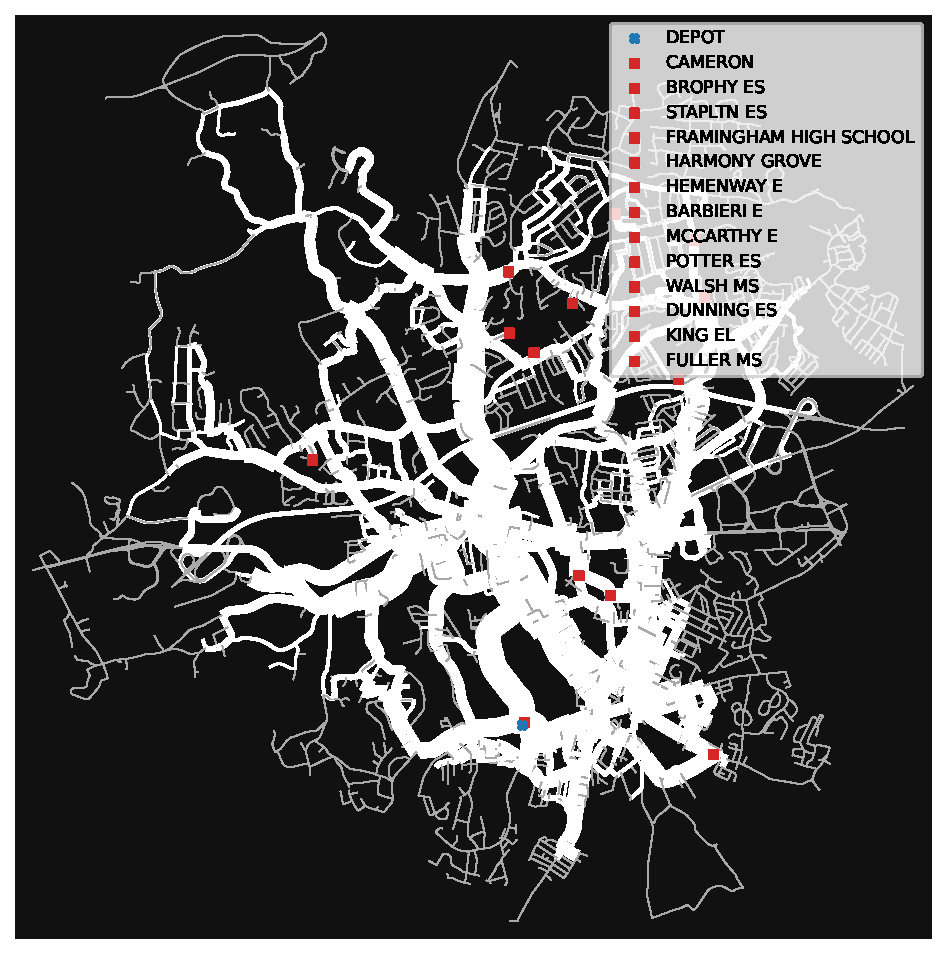
\includegraphics[width=0.99\textwidth, alt={Route-density map of current \glsfullentry{fps} bus routes. White road links indicate roads used by more buses, with selected route segments highlighted in red.}]{figures/existing_routes.pdf}
        \subcaption{Current routes used by \gls{fps}}
    \end{subfigure}
    \begin{subfigure}{0.32\textwidth}
        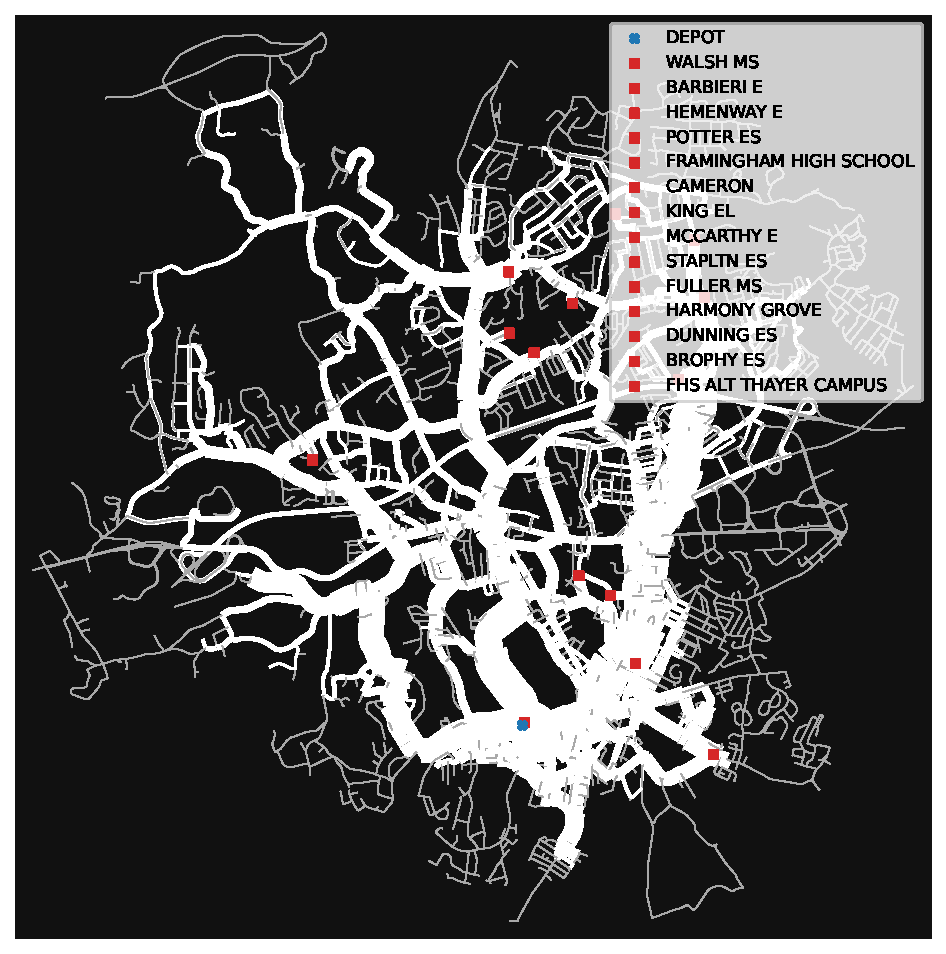
\includegraphics[width=0.99\textwidth, alt={Route-density map of proposed routes generated using \glsfullentry{bra}. White road links indicate roads used by more buses, with selected route segments highlighted in red.}]{figures/bird_assigned_students_routes.pdf}
        \subcaption{Proposed routes generated using \gls{bra}}
    \end{subfigure}
    \begin{subfigure}{0.32\textwidth}
        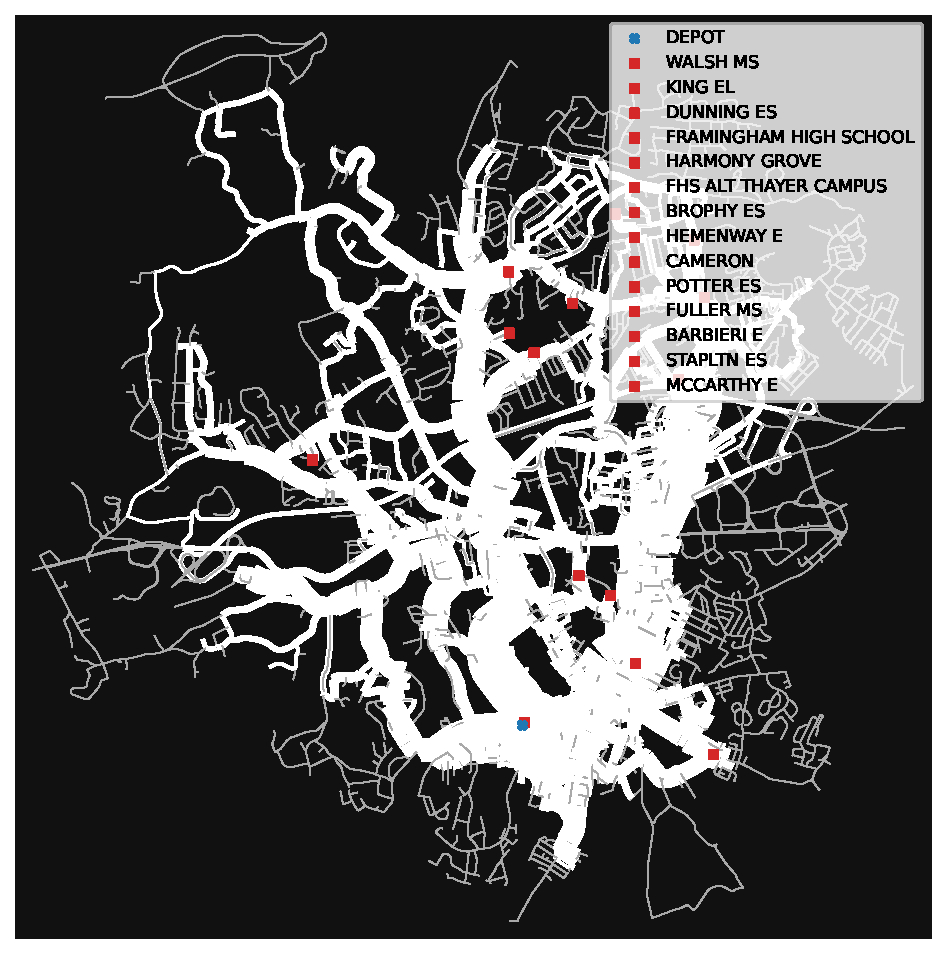
\includegraphics[width=0.99\textwidth, alt={Route-density map of possible routing for students at least 1.5 miles from school. White road links indicate roads used by more buses, with selected route segments highlighted in red.}]{figures/bird_all_students_over_1_5_miles.pdf}
        \subcaption{Possible routing of students $\geq$ 1.5 miles away}
    \end{subfigure}
    \caption{Visualization of routes, with each road link represented by how many buses travel along it.}
    \label{fig:routes}
\end{figure}

Additionally, \gls{fps} is moving from an opt-in routing model to an opt-out model, where students are provided transport by default. Thus, I applied \gls{bra} with the current fleet constraints and found that the current student population living over 1.5 miles\footnote{As mentioned in \autoref{sec:existing_routes}, \gls{fps} is required under Massachusetts law to offer no-cost transportation for students living over 2 miles away. However, as of writing, \gls{fps} also offers bus transportation for students living between 1 and 2 miles away for an associated fee \cite{framinghampublicschoolsRider, framinghamschoolcommittee2022Student}.} from their school can be served using the existing fleet available to \gls{fps}. Conversely, all students in the district with the current bus fleet cannot be fully served with the assumed modeling and operational constraints, as shown in \autoref{tab:travel_times_all}. While these preliminary results are directional and should be further refined, they demonstrate how \gls{fps} can substantially change their bus routing to serve a greater number of students while improving average travel-time outcomes under the modeled assumptions.

\begin{table}[!htbp]
    \centering
    \begin{tabular}{@{}lllllllll@{}}
        \toprule
         Served & \multicolumn{4}{l}{\textbf{All Students $\geq$ 1.5 miles away}} & \multicolumn{4}{l}{\textbf{All students}} \\
         & Mean & StDev & Min & Max & Mean & StDev & Min & Max \\ \midrule
         All students 
         & 30.81 & 14.67 & 3.52 & 59.62 
         & 29.67 & 14.95 & 0.73 & 59.76 \\
         Non-English at home 
         & 31.69 & 14.49 & 3.55 & 59.62 
         & 30.77 & 14.47 & 0.73 & 59.43 \\
         Non-car owning household 
         & 32.24 & 14.00 & 4.60 & 59.62 
         & 31.68 & 14.41 & 2.41 & 59.76 \\
         Students with disabilities 
         & 29.93 & 14.37 & 4.55 & 58.26 
         & 30.52 & 15.03 & 2.14 & 59.76
         \\ \midrule 
         Total number of students & \multicolumn{4}{l}{6304} & \multicolumn{4}{l}{8210} \\
         Students unassigned & \multicolumn{4}{l}{0} & \multicolumn{4}{l}{13} \\ 
         Buses used & \multicolumn{4}{l}{62} & \multicolumn{4}{l}{78} \\
         \bottomrule
    \end{tabular}
    \caption{Estimated travel times of students in minutes with different routing configurations with the set of all students. Does not account for intersection delay, assumes constant bus speed.}
    \label{tab:travel_times_all}
\end{table}

The Pareto fronts in \autoref{fig:pareto} summarize the tradeoffs induced by varying resource limits and objective weights in the \gls{bra} candidate-selection model. Each point represents a feasible routing configuration generated under the same data assumptions but with different priorities over fleet use, coverage, and student travel time. I also analyze the current \gls{fps} routing plan as a baseline design, making it easy to assess whether existing operations are dominated by generated alternatives under the modeled constraints. Because travel times are estimated using simplified speed assumptions rather than calibrated \gls{avl} data, these fronts should be interpreted as relative planning comparisons rather than final operational schedules.

\begin{figure}[!htbp]
    \centering
    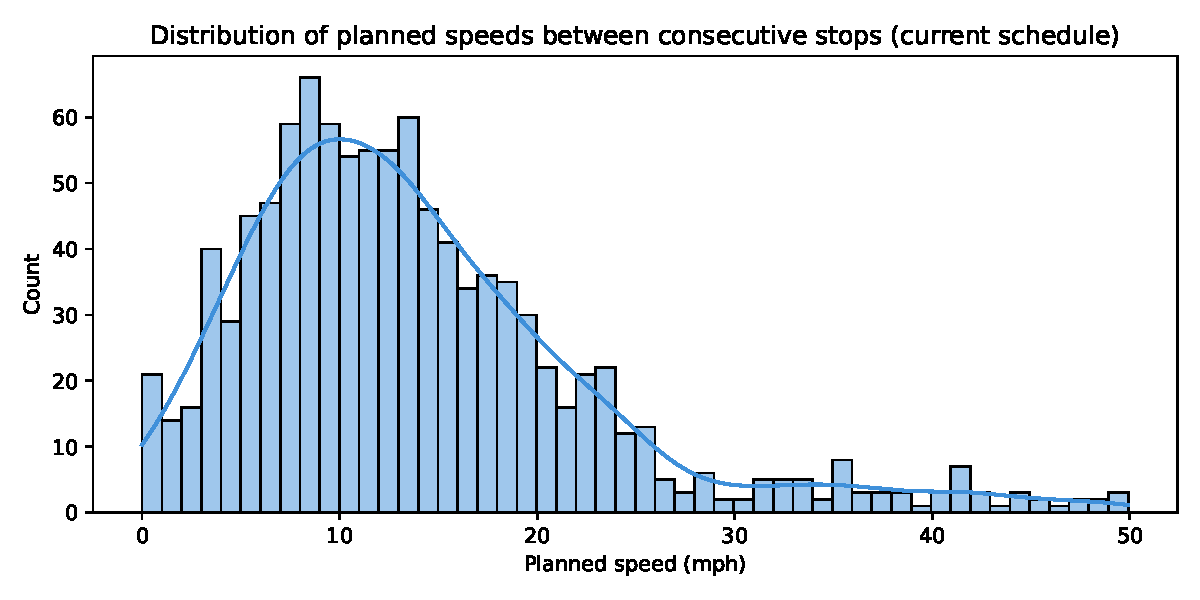
\includegraphics[width=0.99\textwidth, alt={Histogram of implied planned bus speeds between consecutive stops, measured in kilometers per hour. Most stop-to-stop segments fall between about 5 and 20 km/h, with the highest concentration around 10 to 15 km/h and a long right tail extending toward 50 km/h, indicating substantial variation in planned travel speeds.}]{figures/current_schedule_speed_distribution.pdf}
    \caption{Distribution of implied planned speeds between consecutive stops in the existing route data. Speeds are calculated from planned stop-to-stop movements and show substantial variation across route segments.}
    \label{fig:planned-speed-distribution}
\end{figure}

Although the \gls{bra} experiments use a constant-speed assumption for travel-time estimation, the existing route data suggest that planned bus speeds vary substantially across stop-to-stop segments. \autoref{fig:planned-speed-distribution} shows that most implied planned speeds are well below free-flow arterial speeds, with a long right tail of faster segments. This reinforces that the results should be interpreted as comparative planning estimates rather than deployment-ready schedules, and that future work should calibrate travel times using \gls{avl} traces or a time-dependent routing engine.

\begin{figure}[!htbp]
    \centering
    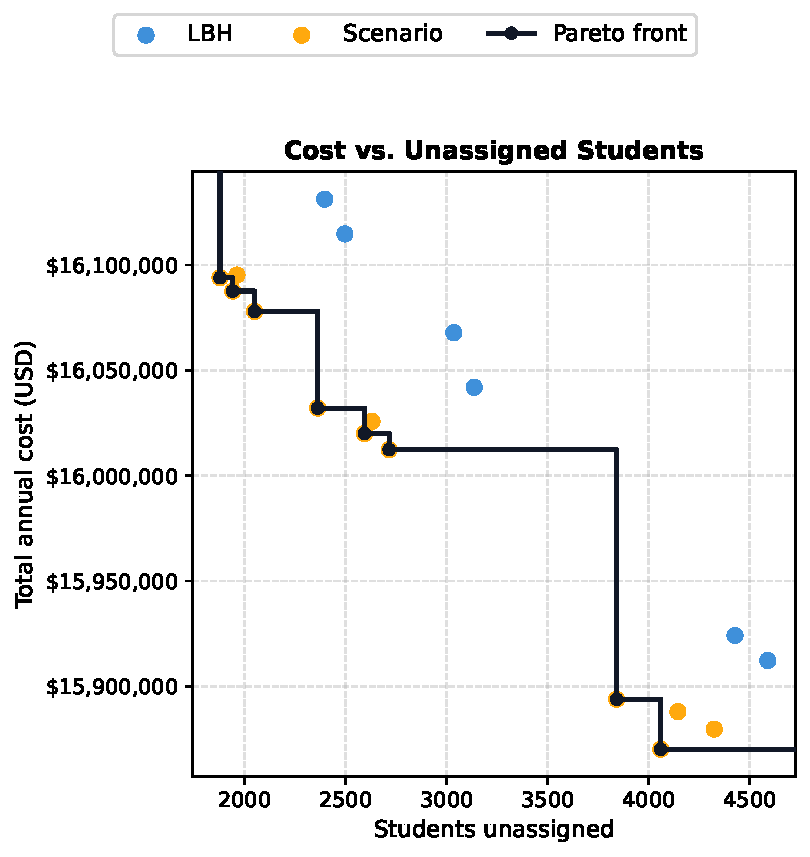
\includegraphics[width=0.495\linewidth, alt={Scatter plot of total annual cost versus students assigned for \glsfullentry{bird} testing data. \glsfullentry{lbh} and Scenario solutions are plotted to compare how stop usage affects cost.}]{figures/routing_bird_mcdp_pareto_routing_simple_caps_cost_unassigned.pdf}
    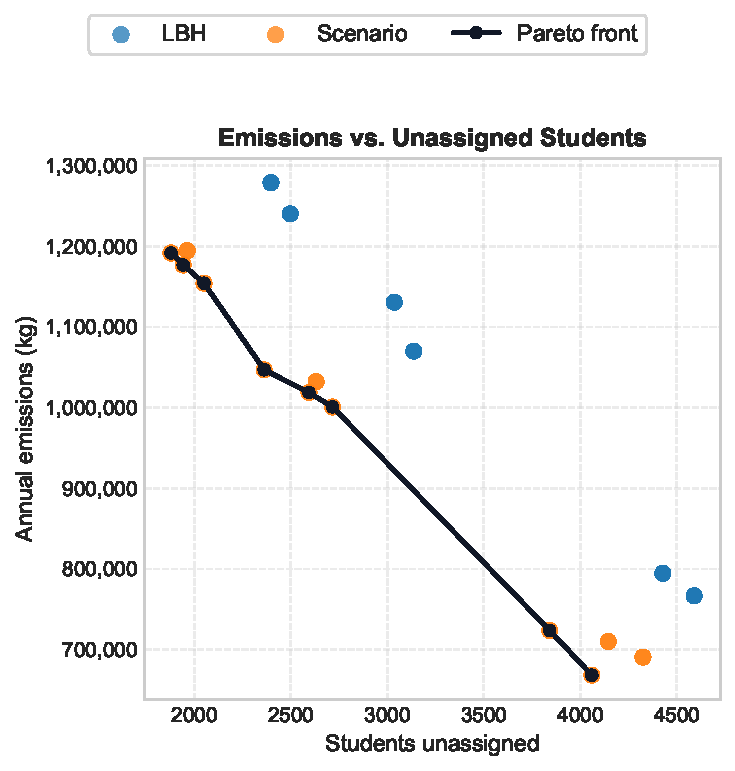
\includegraphics[width=0.495\linewidth, alt={Scatter plot of total annual cost versus students assigned for \glsfullentry{bird} testing data. \glsfullentry{lbh} and Scenario solutions are plotted, with the Pareto frontier showing the best emission-coverage tradeoff.}]{figures/routing_bird_mcdp_pareto_routing_simple_caps_emissions_unassigned.pdf}
    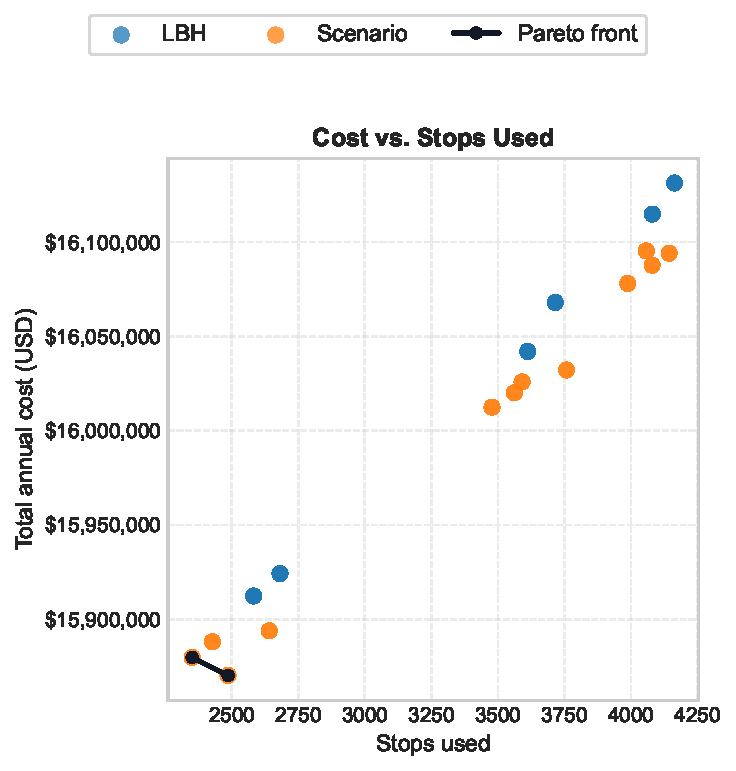
\includegraphics[width=0.495\linewidth, alt={Scatter plot of total annual cost versus students assigned for \glsfullentry{bird} testing data. \glsfullentry{lbh} and Scenario solutions are plotted, with the Pareto frontier showing the best cost-coverage tradeoff.}]{figures/routing_bird_mcdp_pareto_routing_simple_caps_cost_stops.pdf}
    \caption{Pareto fronts for \gls{bra} simplified routing configuration with student data. Each point on these fronts is a valid solution of the co‑design problem with different resource allocations among \gls{mdpi} components (fleet, driver, monitor, fuel, maintenance). The figure makes visible the planning tradeoffs implied by the categorical composition.}
    \label{fig:pareto}
\end{figure}

To refine these results further, future work will require \gls{fps} to provide a unified student-level dataset linking each student's home location, school, grade, transportation eligibility, current stop assignment, bus assignment, disability status, wheelchair-accessibility requirement where applicable, and any district-specific service constraints. Additionally, I would like to confirm whether routing should use district-approved stops or allow \gls{bra} to generate new stop assignments, and also whether demographic equity constraints should be embedded directly into the \gls{bra} optimization using a strategy similar to \textcite{paviaDesigningEquitableTransit2023}.

As this work is continued, one should define service standards that should govern implementation, including maximum ride time, maximum walk distance to stops, arrival windows, and treatment of students with disabilities and accessibility needs. Future work should replace constant-speed assumptions with calibrated travel times that reflect road type, congestion, and school-period traffic conditions.
